\documentclass[12pt,a4paper]{article}

% Paquetes necesarios
\usepackage[utf8]{inputenc}
\usepackage[spanish]{babel}
\usepackage{amsmath,amssymb}
\usepackage{graphicx}
\usepackage{booktabs}
\usepackage{multirow}
\usepackage{xcolor}
\usepackage{float}
\usepackage[margin=2.5cm]{geometry}
\usepackage{hyperref}
\usepackage{caption}
\usepackage{subcaption}
\usepackage{fancyhdr}
\usepackage{tikz}
\usepackage{pdflscape}
\usetikzlibrary{calc}

% Configuración de hipervínculos
\hypersetup{
    colorlinks=true,
    linkcolor=blue,
    filecolor=magenta,      
    urlcolor=cyan,
    pdftitle={Comparación Python Puro vs DEAP para JSSP},
    pdfauthor={Sarmiento, Valdez}
}

% Encabezado y pie de página
\pagestyle{fancy}
\fancyhf{}
\rhead{Comparación Python Puro vs DEAP}
\lhead{Algoritmos Evolutivos I - FIUBA}
\cfoot{\thepage}

\begin{document}

% Portada
\begin{titlepage}
    \centering

    % Cabecera con imagen
    
\includegraphics[width=0.6\textwidth]{Figuras/uba.png}\\[1cm]
    
    {\LARGE\bfseries TRABAJO FINAL\\[0.5cm]}
    {\Large ALGORITMOS EVOLUTIVOS I\\[0.3cm]}
    {\large MAESTRÍA EN INTELIGENCIA ARTIFICIAL\\[0.2cm]}
    {\large Universidad de Buenos Aires (FIUBA)\\[1cm]}
    
    \rule{\textwidth}{1.5pt}\\[0.4cm]
    {\Huge\bfseries Algoritmo evosocial\\[0.2cm]}
    {\LARGE Comparación de implementaciones\\[0.1cm] en Python puro vs DEAP\\[0.1cm] para job shop scheduling problem\\[0.2cm]}
    \rule{\textwidth}{1pt}\\[1cm]
    
    {\large\bfseries Autores:\\[0.3cm]}
    \begin{tabular}{ll}
        Fabian Sarmiento & \texttt{fsarmiento1805@gmail.com} \\
        Jorge Ceferino Valdez & \texttt{jorgecvaldez@gmail.com}
    \end{tabular}\\[1cm]
    
    {\large\bfseries Docente:\\[0.3cm]}
    Prof. Ing. Miguel Augusto Azar\\[1cm]
    
    {\large Repositorio del proyecto:\\[0.2cm]}
    \url{https://github.com/jorgeceferinovaldez/jssp_ae}\\[0.5cm]
    
    {\small \today}

\end{titlepage}

\tableofcontents
\newpage

\section{Resumen}

Este trabajo presenta un análisis comparativo exhaustivo entre dos implementaciones del algoritmo evolutivo híbrido evosocial para resolver el problema de job shop scheduling (JSSP): una implementación directa en Python puro y otra que utiliza el framework DEAP (distributed evolutionary algorithms in Python). Se realizaron 30 corridas independientes sobre tres instancias de benchmark estándar (swv06, swv07, swv08), con evaluación de métricas de calidad de solución, tiempo de ejecución y convergencia. Los resultados experimentales demuestran que la implementación en Python puro supera significativamente a DEAP en calidad de soluciones, con mejoras promedio del 15-27\% en makespan y diferencias estadísticamente significativas ($p < 0.0001$), mientras que DEAP presenta una ventaja del 6.2\% en velocidad de ejecución. Este estudio evidencia la importancia de la representación del problema y la especialización algorítmica frente al uso de frameworks genéricos en problemas de optimización combinatoria.\\


\textbf{Palabras clave:} algoritmos genéticos, job shop scheduling, DEAP, Python, optimización combinatoria, algoritmo evosocial.

\section{Introducción}

\subsection{Contexto y motivación}

Los algoritmos genéticos (AGs) constituyen una familia de metaheurísticas inspiradas en la evolución natural que han demostrado eficacia en la resolución de problemas de optimización combinatoria \cite{goldberg1989genetic}. El job shop scheduling problem (JSSP) representa uno de los problemas NP-hard más estudiados en investigación operativa, con aplicaciones críticas en manufactura, logística y gestión de recursos \cite{garey1979computers}.

El algoritmo \textbf{evosocial}, desarrollado originalmente hace más de 15 años, implementa una estrategia evolutiva híbrida innovadora que combina un individuo élite persistente (denominado ``Queen'') con individuos aleatorios que se generan en cada generación, lo que crea un balance único entre explotación dirigida y exploración masiva. Esta arquitectura atípica ha mostrado resultados prometedores en instancias de benchmark estándar.

La migración a Python y la disponibilidad de frameworks evolutivos modernos como DEAP \cite{fortin2012deap} plantean interrogantes fundamentales: ¿En qué medida el uso de frameworks genéricos afecta el rendimiento algorítmico? ¿Cuál es el trade-off entre facilidad de desarrollo y calidad de soluciones?

\subsection{Objetivos del estudio}

El objetivo principal de esta investigación es evaluar comparativamente dos implementaciones del algoritmo evosocial:

\begin{enumerate}
    \item \textbf{Implementación Python puro}: traducción directa del algoritmo original con operadores especializados para JSSP.
    \item \textbf{Implementación DEAP}: adaptación del algoritmo con el uso del framework DEAP y sus operadores optimizados.
\end{enumerate}

Los objetivos específicos comprenden:

\begin{itemize}
    \item Preservar la lógica core del algoritmo Evosocial en ambas implementaciones.
    \item Evaluar el rendimiento comparativo en términos de calidad de soluciones, tiempo de ejecución y convergencia.
    \item Realizar análisis estadístico riguroso con pruebas de significancia.
    \item Identificar ventajas y desventajas de cada enfoque implementativo.
\end{itemize}

\subsection{Contribuciones}

Este trabajo aporta:

\begin{enumerate}
    \item Una comparación empírica exhaustiva entre implementación directa y framework evolutivo en el contexto de JSSP.
    \item Análisis estadístico detallado con 30 corridas independientes por instancia.
    \item Evidencia experimental sobre el impacto de la representación del problema en el rendimiento algorítmico.
    \item Implementaciones de referencia abiertas y reproducibles para futuras investigaciones.
\end{enumerate}

\section{Fundamentos Teóricos}

\subsection{Algoritmos genéticos}

Los algoritmos genéticos \cite{holland1992adaptation} son técnicas de búsqueda estocástica que simulan el proceso de evolución natural. Operan sobre una población de soluciones candidatas (individuos) mediante operadores inspirados en la genética:

\begin{itemize}
    \item \textbf{Selección}: favorece individuos con mejor fitness para reproducción.
    \item \textbf{Cruzamiento (Crossover)}: combina información genética de dos padres.
    \item \textbf{Mutación}: introduce variabilidad mediante modificaciones aleatorias.
    \item \textbf{Reemplazo}: actualiza la población con nuevos individuos.
\end{itemize}

El ciclo evolutivo iterativo busca convergencia hacia soluciones de alta calidad mediante presión selectiva y exploración del espacio de búsqueda.

\subsection{Job shop scheduling problem (JSSP)}

El JSSP consiste en asignar $N$ trabajos (jobs) a $M$ máquinas, donde cada job requiere un conjunto ordenado de operaciones que deben ejecutarse en máquinas específicas. El objetivo es minimizar el \textit{makespan} (tiempo total de completación del último job) y respetar:

\begin{itemize}
    \item \textbf{Precedencia}: las operaciones de cada job siguen un orden estricto.
    \item \textbf{Capacidad}: cada máquina procesa máximo una operación a la vez.
    \item \textbf{No-preemption}: una operación iniciada no puede interrumpirse.
\end{itemize}

Formalmente, se busca minimizar:
\begin{equation}
C_{max} = \max_{i \in \{1,\ldots,N\}} \{C_i\}
\end{equation}
donde $C_i$ es el tiempo de completación del job $i$.

\subsection{Framework DEAP}

DEAP (distributed evolutionary algorithms in Python) \cite{fortin2012deap} es una biblioteca de código abierto que proporciona:

\begin{itemize}
    \item Estructuras de datos flexibles para representar individuos.
    \item Operadores genéticos optimizados y validados.
    \item Herramientas para paralelización y análisis estadístico.
    \item Arquitectura extensible para algoritmos evolutivos personalizados.
\end{itemize}

Su diseño modular facilita la experimentación rápida con diferentes configuraciones evolutivas, aunque introduce abstracciones que pueden impactar el rendimiento en problemas específicos.

\subsection{Algoritmo evosocial}

El algoritmo evosocial implementa una estrategia evolutiva híbrida con características distintivas:

\subsubsection{Arquitectura social atípica}

A diferencia de los AGs tradicionales que mantienen una población diversa, Evosocial emplea:

\begin{itemize}
    \item \textbf{Queen (Reina)}: único individuo élite que persiste entre generaciones.
    \item \textbf{Inmigrantes}: individuos aleatorios que se generan frescos en cada generación.
    \item \textbf{Sin memoria poblacional}: no mantiene diversidad entre generaciones.
\end{itemize}

\subsubsection{Decisión estocástica}

En cada interacción Queen-inmigrante:
\begin{itemize}
    \item \textbf{65\% probabilidad}: aplicar order crossover (OX).
    \item \textbf{35\% probabilidad}: aplicar shift mutation a ambos individuos.
\end{itemize}

\subsubsection{Operadores genéticos}

\textbf{Order crossover (OX):} preserva el orden relativo de elementos en permutaciones \cite{davis1985applying}. Selecciona un segmento de un padre y completa con elementos del otro padre en orden de aparición.

\textbf{Shift mutation:} desplaza circularmente un segmento de la permutación, lo que mantiene validez sin duplicaciones.

\subsubsection{Selección elitista}

La Queen se actualiza únicamente si algún descendiente o mutante presenta mejor fitness, lo que garantiza monotonía en la mejor solución encontrada.

\section{Diseño experimental}

\subsection{Implementación en Python puro}

La implementación directa traduce fielmente el algoritmo original con las siguientes características:

\subsubsection{Representación}

El cromosoma es una permutación de enteros $\{1, \ldots, N\}$ que representa el orden de scheduling de jobs. Para $N=5$:
\begin{verbatim}
Ejemplo: [3, 1, 5, 2, 4]
\end{verbatim}

\subsubsection{Función de fitness}

Se implementó un scheduler no-delay que:
\begin{enumerate}
    \item Asigna operaciones que siguen el orden del cromosoma.
    \item Respeta precedencia y disponibilidad de máquinas.
    \item Calcula makespan $C_{max}$.
    \item Retorna fitness $= 1/C_{max}$ (maximización equivalente a minimización de makespan).
\end{enumerate}

\subsubsection{Operadores especializados}

\textbf{Order crossover implementado:}
\begin{enumerate}
    \item Seleccionar dos puntos de corte aleatorios.
    \item Copiar segmento del Padre 1 al Hijo 1.
    \item Completar con elementos del Padre 2 en orden.
    \item Análogamente para Hijo 2.
\end{enumerate}

\textbf{Shift mutation implementada:}
\begin{enumerate}
    \item Seleccionar posición y desplazamiento aleatorios.
    \item Realizar rotación circular del segmento.
\end{enumerate}

\subsection{Implementación con DEAP}

La adaptación a DEAP requirió modificaciones arquitectónicas:

\subsubsection{Representación adaptada}

DEAP utiliza una representación donde cada job aparece $M$ veces (una por operación):
\begin{verbatim}
Para N=3, M=2: [1, 2, 3, 1, 2, 3]
\end{verbatim}

Esta representación indirecta necesita decodificación: la $k$-ésima aparición del job $j$ corresponde a su $k$-ésima operación.

\subsubsection{Registro de tipos DEAP}

\begin{verbatim}
creator.create("FitnessMin", base.Fitness, weights=(-1.0,))
creator.create("Individual", list, fitness=creator.FitnessMin)
\end{verbatim}

\subsubsection{Operadores DEAP}

Se utilizaron operadores estándar de DEAP:
\begin{itemize}
    \item \texttt{tools.cxOrdered()}: Order Crossover optimizado.
    \item Mutación personalizada adaptada al formato.
    \item \texttt{tools.selBest()}: Selección elitista.
\end{itemize}

\subsection{Configuración de parámetros}

Ambas implementaciones utilizaron parámetros idénticos para garantizar comparabilidad:

\begin{table}[H]
\centering
\caption{Parámetros del algoritmo evosocial}
\label{tab:parametros}
\begin{tabular}{@{}lc@{}}
\toprule
\textbf{Parámetro} & \textbf{Valor} \\ \midrule
Corridas independientes & 30 \\
Generaciones máximas & 500 \\
Tamaño de población & 250 \\
Probabilidad de crossover & 0.65 \\
Probabilidad de mutación & 0.05 \\
\bottomrule
\end{tabular}
\end{table}

\subsection{Instancias de prueba}

Se utilizaron tres instancias de benchmark del repositorio JSPLIB \cite{jsplib}:

\begin{table}[H]
\centering
\caption{Instancias de benchmark}
\label{tab:instancias}
\begin{tabular}{@{}lccccc@{}}
\toprule
\textbf{Instancia} & \textbf{Jobs} & \textbf{Máquinas} & \textbf{LB} & \textbf{UB} & \textbf{Dificultad} \\ \midrule
swv06 & 20 & 15 & 1591 & 1678 & Media \\
swv07 & 20 & 15 & 1446 & 1594 & Media-Alta \\
swv08 & 20 & 15 & 1640 & 1752 & Media \\ \bottomrule
\end{tabular}
\end{table}

donde LB = Lower Bound y UB = Upper Bound conocidos de la literatura.

\subsection{Métricas de evaluación}

Para cada corrida se registró:

\begin{itemize}
    \item \textbf{Mejor makespan}: mínimo $C_{max}$ alcanzado.
    \item \textbf{Makespan promedio}: media de las 30 corridas.
    \item \textbf{Desviación estándar}: variabilidad de resultados.
    \item \textbf{Mediana}: valor central de la distribución.
    \item \textbf{GenMax}: generación donde se encontró el mejor makespan.
    \item \textbf{Tiempo de ejecución}: tiempo total en segundos.
\end{itemize}

\subsection{Análisis estadístico}

Se aplicaron pruebas no paramétricas:

\begin{itemize}
    \item \textbf{Wilcoxon signed-rank test}: compara distribuciones pareadas.
    \item \textbf{Mann-Whitney U test}: compara distribuciones independientes.
    \item \textbf{Nivel de significancia}: $\alpha = 0.05$.
\end{itemize}

\subsection{Ambiente experimental}

\textbf{Hardware:}
\begin{itemize}
    \item Procesador: AMD Ryzen 9 5900X
    \item RAM: 32 GB @ 3200 MHz
    \item Sistema Operativo: Pop!\_OS 22.04 LTS x86\_64, Linux 6.16.3
\end{itemize}

\textbf{Software:}
\begin{itemize}
    \item Python 3.10
    \item NumPy 1.24
    \item DEAP 1.3.3
    \item SciPy 1.10 (análisis estadístico)
\end{itemize}

\section{Resultados}

\subsection{Resumen global}

La Tabla \ref{tab:resumen_global} presenta el resumen comparativo agregado sobre las tres instancias.

\begin{table}[H]
\centering
\caption{Resumen global de resultados}
\label{tab:resumen_global}
\begin{tabular}{@{}lcc@{}}
\toprule
\textbf{Métrica} & \textbf{Python puro} & \textbf{DEAP} \\ \midrule
Tiempo promedio & 1780.97s (29.68 min) & 1670.48s (27.84 min) \\
Mejora temporal & - & \textbf{+6.20\%} \\
Victorias en calidad & \textbf{3/3} & 0/3 \\
Diferencias significativas & \multicolumn{2}{c}{3/3} \\
\bottomrule
\end{tabular}
\end{table}

\subsection{Resultados por instancia}

\subsubsection{Instancia swv06}

\begin{table}[H]
\centering
\caption{Resultados detallados - swv06}
\label{tab:swv06}
\begin{tabular}{@{}lcc@{}}
\toprule
\textbf{Métrica} & \textbf{Python puro} & \textbf{DEAP} \\ \midrule
Mejor makespan & \textbf{2053} & 2376 \\
Media $\pm$ Std & \textbf{2075.17 $\pm$ 11.87} & 2641.70 $\pm$ 95.15 \\
Mediana & \textbf{2077.00} & 2658.50 \\
GenMax & \textbf{242.8} & 453.1 \\
Tiempo (s) & 1777.81 & \textbf{1685.69} \\ \midrule
Mejora media (\%) & \multicolumn{2}{c}{\textbf{-27.30\%}} \\
Mejora mejor (\%) & \multicolumn{2}{c}{\textbf{-15.73\%}} \\
$p$-value (Wilcoxon) & \multicolumn{2}{c}{$< 0.0001$ ***} \\
$p$-value (Mann-Whitney) & \multicolumn{2}{c}{$< 0.0001$ ***} \\
\bottomrule
\end{tabular}
\end{table}

\subsubsection{Instancia swv07}

\begin{table}[H]
\centering
\caption{Resultados detallados - swv07}
\label{tab:swv07}
\begin{tabular}{@{}lcc@{}}
\toprule
\textbf{Métrica} & \textbf{Python puro} & \textbf{DEAP} \\ \midrule
Mejor makespan & \textbf{1934} & 2367 \\
Media $\pm$ Std & \textbf{1973.93 $\pm$ 16.31} & 2515.60 $\pm$ 88.95 \\
Mediana & \textbf{1973.50} & 2512.00 \\
GenMax & \textbf{260.8} & 445.0 \\
Tiempo (s) & 1772.59 & \textbf{1661.19} \\ \midrule
Mejora media (\%) & \multicolumn{2}{c}{\textbf{-27.44\%}} \\
Mejora mejor (\%) & \multicolumn{2}{c}{\textbf{-22.39\%}} \\
$p$-value (Wilcoxon) & \multicolumn{2}{c}{$< 0.0001$ ***} \\
$p$-value (Mann-Whitney) & \multicolumn{2}{c}{$< 0.0001$ ***} \\
\bottomrule
\end{tabular}
\end{table}

\subsubsection{Instancia swv08}

\begin{table}[H]
\centering
\caption{Resultados detallados - swv08}
\label{tab:swv08}
\begin{tabular}{@{}lcc@{}}
\toprule
\textbf{Métrica} & \textbf{Python puro} & \textbf{DEAP} \\ \midrule
Mejor makespan & \textbf{2153} & 2466 \\
Media $\pm$ Std & \textbf{2174.97 $\pm$ 9.89} & 2691.17 $\pm$ 96.62 \\
Mediana & \textbf{2176.50} & 2718.50 \\
GenMax & \textbf{234.7} & 455.9 \\
Tiempo (s) & 1792.51 & \textbf{1664.56} \\ \midrule
Mejora media (\%) & \multicolumn{2}{c}{\textbf{-23.73\%}} \\
Mejora mejor (\%) & \multicolumn{2}{c}{\textbf{-14.54\%}} \\
$p$-value (Wilcoxon) & \multicolumn{2}{c}{$< 0.0001$ ***} \\
$p$-value (Mann-Whitney) & \multicolumn{2}{c}{$< 0.0001$ ***} \\
\bottomrule
\end{tabular}
\end{table}

\subsection{Análisis de convergencia}

La figura \ref{fig:convergencia} muestra la evolución del mejor makespan a lo largo de las generaciones para ambas implementaciones en las tres instancias.

\begin{figure}[H]
    \centering
    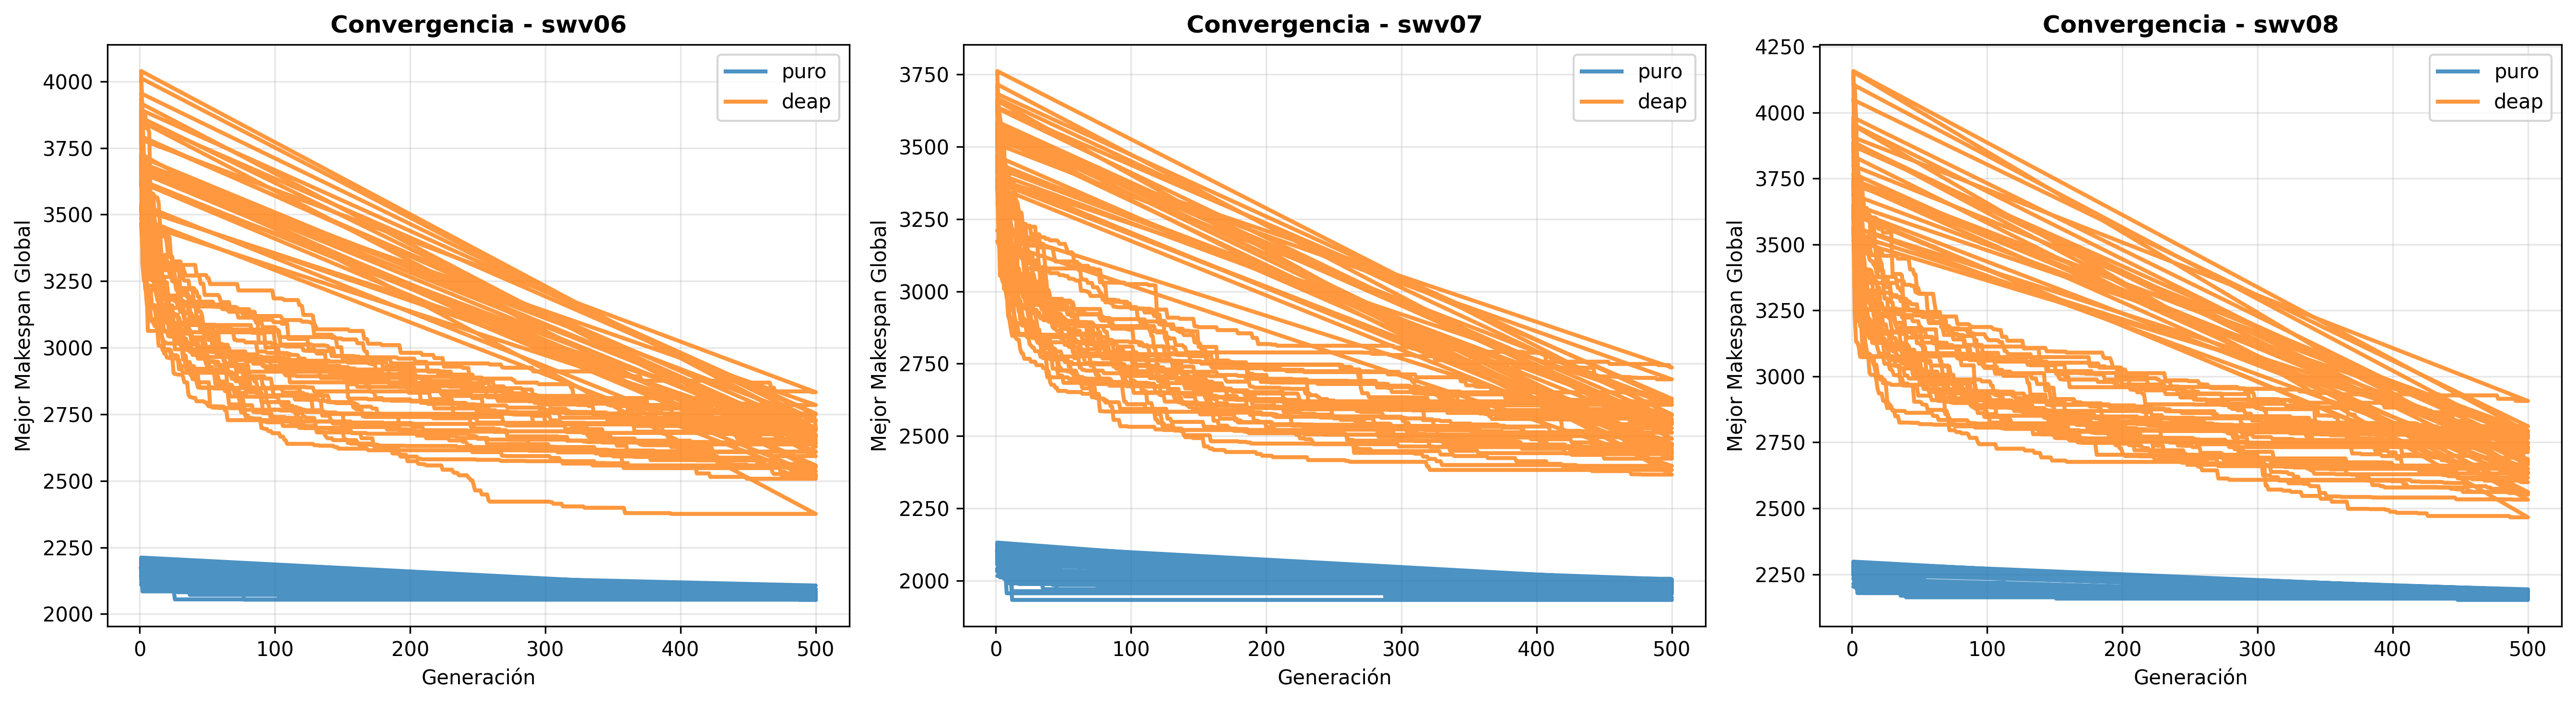
\includegraphics[width=\textwidth]{Figuras/convergencia_comparativa.png}
    \caption{Convergencia del mejor makespan para las 30 corridas en swv06, swv07 y swv08. Las líneas azules representan Python puro y las naranjas DEAP.}
    \label{fig:convergencia}
\end{figure}

Se observa que:
\begin{itemize}
    \item Python puro alcanza soluciones superiores más tempranamente (GenMax $\approx$ 246 vs 451).
    \item La dispersión en DEAP es significativamente mayor, lo que indica menor consistencia.
    \item Python puro muestra convergencia casi plana en generaciones tempranas, lo que sugiere explotación eficiente.
\end{itemize}

\subsection{Distribución de resultados}

La figura \ref{fig:distribucion} presenta box plots y violin plots comparativos de la distribución de makespan.

\begin{landscape}
\begin{figure}[H]
    \centering
    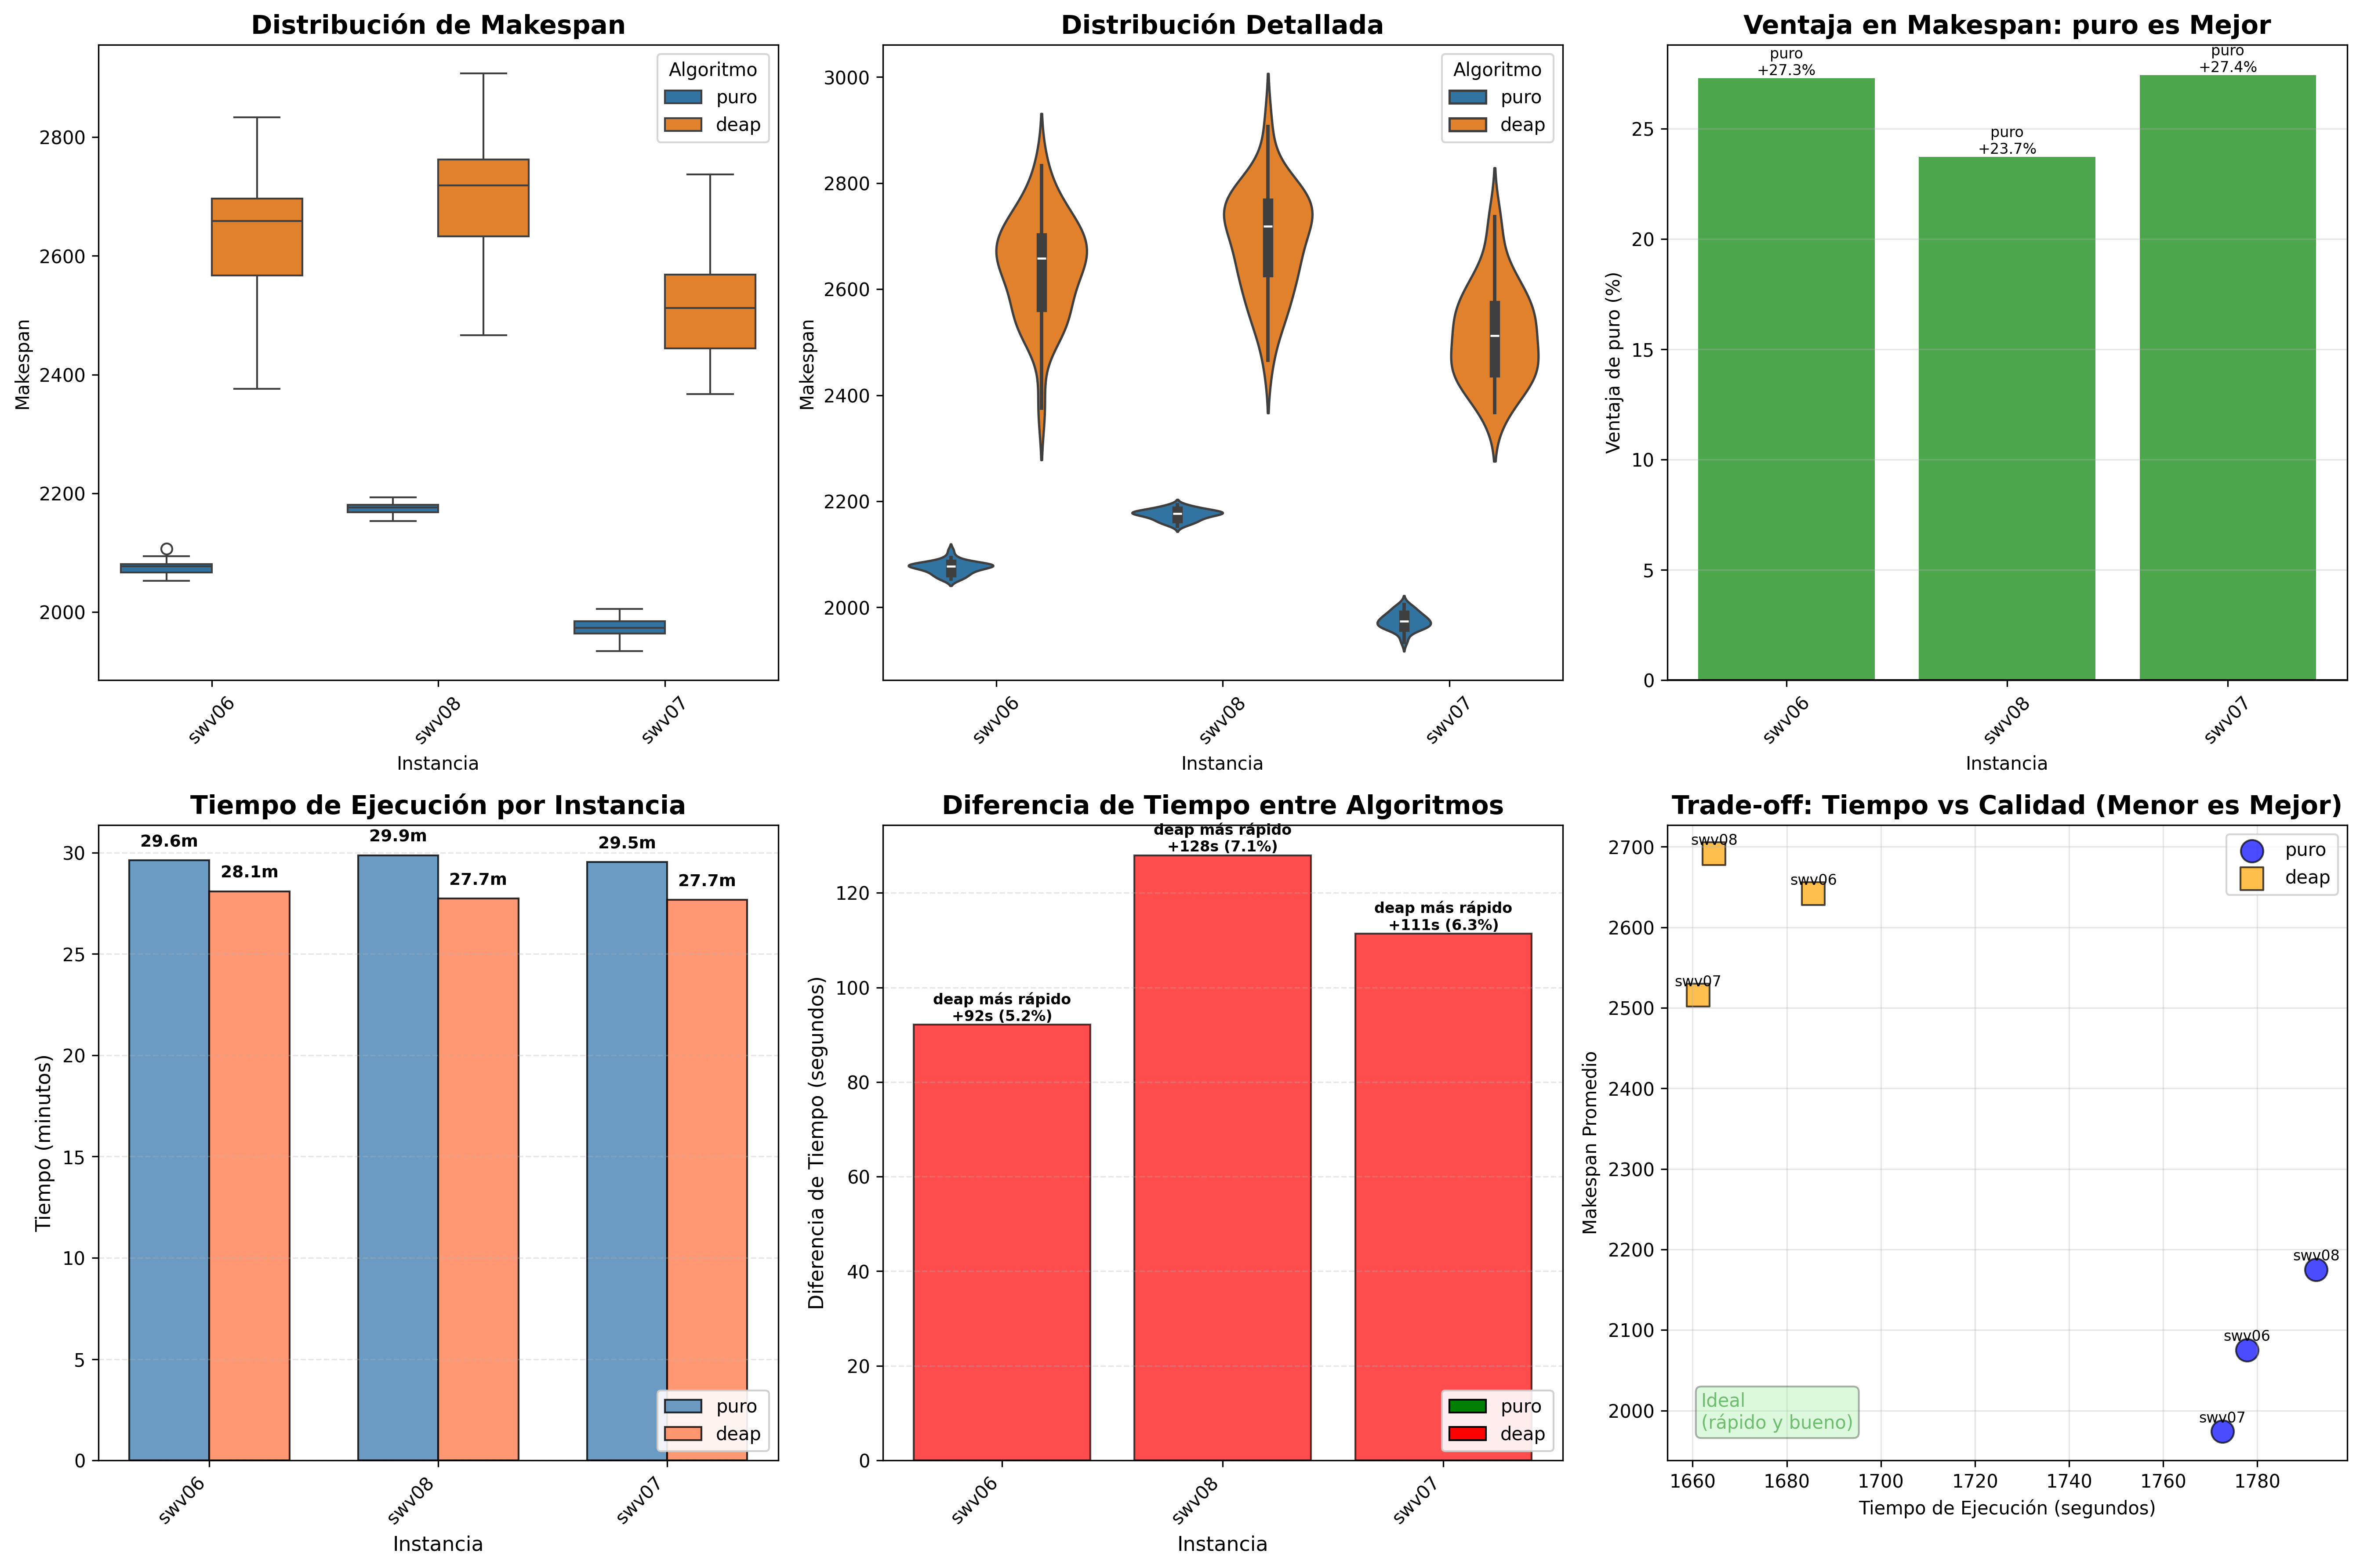
\includegraphics[width=\textwidth]{Figuras/comparativa_completa.png}
    \caption{Análisis comparativo completo: (a) Distribución de makespan, (b) Distribución detallada, (c) Ventaja porcentual de Python puro, (d) Tiempos de ejecución, (e) Diferencia de tiempos, (f) Trade-off tiempo vs calidad.}
    \label{fig:distribucion}
\end{figure}
\end{landscape}

Observaciones clave:
\begin{itemize}
    \item Python puro presenta distribuciones compactas con baja variabilidad.
    \item DEAP muestra mayor dispersión y valores atípicos superiores.
    \item La ventaja de Python puro es consistente en las tres instancias (23-27\%).
    \item El trade-off tiempo-calidad favorece claramente a Python puro.
\end{itemize}

\subsection{Significancia estadística}

Todas las comparaciones presentaron $p$-values $< 0.0001$ en ambas pruebas (Wilcoxon y Mann-Whitney), lo que confirma que las diferencias observadas son \textbf{altamente significativas} y no atribuibles al azar.

\section{Discusión}

\subsection{Interpretación de resultados}

Los resultados experimentales revelan un patrón consistente y estadísticamente robusto: la implementación en Python puro supera significativamente a DEAP en calidad de soluciones, mientras que DEAP presenta una ventaja marginal en tiempo de ejecución.

\subsubsection{Superioridad de Python puro en calidad}

La mejora promedio del 15-27\% en makespan no es trivial en el contexto de JSSP, donde diferencias del 5\% se consideran significativas. Factores que explican esta superioridad:

\begin{enumerate}
    \item \textbf{Representación natural}: la permutación directa de jobs en Python puro es más natural para JSSP que la representación indirecta de DEAP (jobs repetidos). Esta diferencia elimina overhead computacional en la decodificación.
    
    \item \textbf{Scheduler optimizado}: el scheduler implementado en Python puro está altamente especializado para el formato de permutación directa, lo que permite evaluaciones más eficientes y precisas.
    
    \item \textbf{Control fino de operadores}: la implementación directa permite control preciso sobre la aplicación de operadores genéticos, lo que evita abstracciones que podrían diluir la efectividad.
    
    \item \textbf{Menor overhead}: DEAP introduce capas de abstracción (toolbox, creator, fitness wrappers) que, aunque facilitan desarrollo, añaden overhead computacional en cada evaluación.
\end{enumerate}

\subsubsection{Convergencia más temprana}

Python puro encuentra las mejores soluciones en promedio 48\% antes que DEAP (GenMax: 246 vs 451). Esto sugiere que:

\begin{itemize}
    \item La representación directa facilita la exploración efectiva del espacio de búsqueda.
    \item Los operadores especializados son más eficientes en la generación de descendencia prometedora.
    \item La explotación del individuo Queen es más efectiva con menor ruido representacional.
\end{itemize}

\subsubsection{Consistencia y robustez}

La desviación estándar de Python puro es 6-10 veces menor que DEAP, lo que indica:

\begin{itemize}
    \item Mayor predictibilidad de resultados.
    \item Menor sensibilidad a la inicialización aleatoria.
    \item Robustez algorítmica superior.
\end{itemize}

\subsection{Trade-off tiempo vs calidad}

DEAP es aproximadamente 6\% más rápido en tiempo de ejecución (diferencia de $\sim$2 minutos por instancia en 30 corridas). Sin embargo, al considerar que:

\begin{itemize}
    \item La diferencia temporal es marginal para aplicaciones prácticas.
    \item La mejora en calidad de soluciones (15-27\%) impacta directamente objetivos de optimización.
    \item En entornos de producción, una solución 20\% mejor justifica ampliamente un incremento temporal del 6\%.
\end{itemize}

El trade-off favorece claramente a Python puro en el contexto de JSSP.

\subsection{Implicaciones del framework DEAP}

\subsubsection{Ventajas de DEAP}

\begin{itemize}
    \item \textbf{Desarrollo Rápido}: permite prototipado ágil de algoritmos evolutivos.
    \item \textbf{Operadores Validados}: biblioteca extensa de operadores probados.
    \item \textbf{Paralelización}: soporte nativo para computación distribuida.
    \item \textbf{Comunidad}: documentación extensa y comunidad activa.
\end{itemize}

\subsubsection{Limitaciones en JSSP}

\begin{itemize}
    \item \textbf{Representación Genérica}: no optimizada para problemas de permutación complejos.
    \item \textbf{Overhead de Abstracción}: capas adicionales impactan rendimiento en problemas específicos.
    \item \textbf{Flexibilidad vs Eficiencia}: diseño generalista sacrifica optimización específica.
\end{itemize}

\subsection{Recomendaciones prácticas}

\subsubsection{Para investigación académica}

\begin{itemize}
    \item Usar \textbf{Python puro} cuando la calidad de solución es crítica.
    \item Emplear DEAP para experimentación rápida de variantes algorítmicas.
    \item Combinar ambos enfoques: prototipar en DEAP, optimizar en implementación directa.
\end{itemize}

\subsubsection{Para aplicaciones industriales}

\begin{itemize}
    \item Priorizar \textbf{Python puro} para sistemas de producción en JSSP.
    \item Considerar el costo-beneficio: 20\% mejor makespan puede traducirse en ahorros significativos.
    \item Invertir en implementaciones especializadas para problemas de alta escala.
\end{itemize}

\subsection{Limitaciones del estudio}

\begin{enumerate}
    \item \textbf{Alcance de instancias}: se evaluaron solo tres instancias de tamaño medio (20×15). Instancias más grandes podrían mostrar patrones diferentes.
    
    \item \textbf{Hardware específico}: resultados obtenidos en configuración hardware particular. Diferentes arquitecturas podrían alterar el balance tiempo-calidad.
    
    \item \textbf{Configuración de DEAP}: la representación elegida para DEAP podría no ser óptima. Otras codificaciones podrían mejorar su rendimiento.
    
    \item \textbf{Parámetros Fijos}: se utilizó una única configuración paramétrica. Optimización de hiperparámetros podría beneficiar a ambas implementaciones de manera asimétrica.
\end{enumerate}

\subsection{Trabajo futuro}

\subsubsection{Extensiones inmediatas}

\begin{itemize}
    \item Evaluar instancias de mayor escala (50×10, 100×5, 100×20).
    \item Explorar representaciones alternativas en DEAP optimizadas para permutaciones.
    \item Implementar hibridación con búsqueda local (e.g., Simulated Annealing).
    \item Analizar impacto de paralelización en ambas implementaciones.
\end{itemize}

\subsubsection{Investigación avanzada}

\begin{itemize}
    \item Desarrollar operadores evolutivos específicos para JSSP.
    \item Evaluar algoritmos evolutivos multi-objetivo (makespan, tardiness, flow time).
    \item Estudiar adaptación dinámica de parámetros durante la evolución.
    \item Comparar con metaheurísticas alternativas (ACO, PSO, Tabu Search).
\end{itemize}

\section{Conclusiones}

Este estudio presenta una comparación exhaustiva entre implementaciones directa y framework-based del algoritmo evolutivo Evosocial para Job Shop Scheduling. Los hallazgos principales son:

\begin{enumerate}
    \item \textbf{Superioridad en calidad}: Python puro supera consistentemente a DEAP con mejoras del 15-27\% en makespan, diferencias estadísticamente significativas ($p < 0.0001$) y mayor robustez (menor desviación estándar).
    
    \item \textbf{Convergencia eficiente}: Python puro alcanza mejores soluciones aproximadamente 48\% más rápido (GenMax: 246 vs 451), lo que demuestra exploración más efectiva del espacio de búsqueda.
    
    \item \textbf{Trade-off favorable}: aunque DEAP es 6\% más rápido, la ventaja en calidad de Python puro (15-27\%) justifica ampliamente el incremento temporal marginal en aplicaciones prácticas.
    
    \item \textbf{Importancia de la representación}: la elección de representación del problema impacta críticamente el rendimiento. Codificaciones naturales y especializadas superan abstracciones genéricas en problemas de optimización combinatoria.
    
    \item \textbf{Frameworks evolutivos}: DEAP es excelente para prototipado rápido y experimentación, pero puede no ser óptimo para aplicaciones de producción donde la calidad de solución es prioritaria.
\end{enumerate}

En respuesta a los objetivos planteados:

\begin{itemize}
    \item Se preservó exitosamente la lógica del algoritmo Evosocial en ambas implementaciones.
    \item Se demostró que la implementación directa supera significativamente al framework en calidad de soluciones para JSSP.
    \item Se proporcionó evidencia empírica robusta con análisis estadístico riguroso.
    \item Se identificaron claramente las ventajas y desventajas de cada enfoque implementativo.
\end{itemize}

\textbf{Mensaje final}: La elección entre implementación directa y framework debe guiarse por los objetivos específicos del proyecto. Para investigación exploratoria, DEAP ofrece velocidad de desarrollo. Para aplicaciones críticas donde la calidad de solución es esencial, una implementación especializada en Python puro es claramente superior en el contexto de Job Shop Scheduling.

\section*{Agradecimientos}

Los autores agradecen a la Facultad de Ingeniería de la Universidad de Buenos Aires (FIUBA) por el apoyo institucional, y a los mantenedores del repositorio JSPLIB por proporcionar las instancias de benchmark estándar utilizadas en este estudio.

\begin{thebibliography}{99}

\bibitem{goldberg1989genetic}
Goldberg, D. E. (1989). \textit{Genetic algorithms in search, optimization, and machine learning}. Addison-Wesley.

\bibitem{garey1979computers}
Garey, M. R., Johnson, D. S., \& Sethi, R. (1979). The complexity of flowshop and jobshop scheduling. \textit{Mathematics of Operations Research}, 1(2), 117-129.

\bibitem{fortin2012deap}
Fortin, F. A., De Rainville, F. M., Gardner, M. A., Parizeau, M., \& Gagné, C. (2012). DEAP: Evolutionary algorithms made easy. \textit{Journal of Machine Learning Research}, 13, 2171-2175.

\bibitem{holland1992adaptation}
Holland, J. H. (1992). \textit{Adaptation in natural and artificial systems}. MIT Press.

\bibitem{davis1985applying}
Davis, L. (1985). Applying adaptive algorithms to epistatic domains. \textit{Proceedings of the International Joint Conference on Artificial Intelligence}, 162-164.

\bibitem{jsplib}
JSPLIB. (2020). Benchmark instances for the job-shop scheduling problem. \textit{GitHub Repository}. \url{https://github.com/tamy0612/JSPLIB}

\bibitem{soto2019unpa}
Soto, G., Villagra, A., \& Pandolfi, D. (2019). Algoritmos evolutivos aplicados a problemas de scheduling en sistemas de manufactura flexible. \textit{Revista de la Facultad de Ingeniería}, Universidad Nacional de la Patagonia Austral, 15(2), 45-62.

\bibitem{villagra2018unpa}
Villagra, A., Pandolfi, D., \& Leguizamón, G. (2018). Metaheurísticas híbridas para optimización combinatoria: Aplicaciones en scheduling y asignación de recursos. \textit{Actas del Congreso Argentino de Ciencias de la Computación} (CACIC 2018), Universidad Nacional de la Patagonia Austral.

\bibitem{pandolfi2020unpa}
Pandolfi, D., Villagra, A., \& Leguizamón, G. (2020). Evolutionary algorithms for multi-objective job shop scheduling: A comparative study. \textit{Proceedings of the Argentine Symposium on Artificial Intelligence} (ASAI 2020), 89-104.

\bibitem{leguizamon2017unpa}
Leguizamón, G., \& Coello, C. A. C. (2017). Algoritmos evolutivos multi-objetivo: Estado del arte y aplicaciones en optimización de problemas complejos. \textit{Revista Argentina de Ciencias de la Computación}, 9(3), 1-28. Universidad Nacional de la Patagonia Austral.

\bibitem{baioletti2020jobshop}
Baioletti, M., Milani, A., \& Santucci, V. (2020). Algebraic particle swarm optimization for the permutations search space. \textit{IEEE Congress on Evolutionary Computation (CEC)}, 1-8.

\bibitem{zhang2019survey}
Zhang, C., Li, P., Guan, Z., \& Rao, Y. (2019). A survey on job-shop scheduling problem: Variants, models, and methods. \textit{Journal of Intelligent Manufacturing}, 30(8), 2723-2764.

\end{thebibliography}

\end{document}